% =====================================================================
%  CIE 555 - Neural Networks and Deep Learning
%  Project: Grammatical Error Correction on the C4_200M dataset
%  Compile:  pdflatex report.tex   (run twice for the table of contents)
% =====================================================================
\documentclass[11pt,a4paper]{article}

\usepackage[utf8]{inputenc}
\usepackage[T1]{fontenc}
\usepackage[margin=1in]{geometry}
\usepackage{amsmath,amssymb}
\usepackage{graphicx}
\usepackage{booktabs}
\usepackage{array}
\usepackage{caption}
\usepackage{subcaption}
\usepackage{xcolor}
\usepackage{enumitem}
\usepackage{listings}
\usepackage[hidelinks]{hyperref}

\captionsetup{font=small,labelfont=bf}
\setlength{\parskip}{0.4em}
\renewcommand{\arraystretch}{1.25}

\definecolor{boxgray}{gray}{0.95}
\lstset{basicstyle=\ttfamily\small,backgroundcolor=\color{boxgray},
        breaklines=true,frame=single,framesep=4pt,xleftmargin=4pt}

% --------------------------------------------------------------------
\title{\textbf{Grammatical Error Correction on the C4\_200M Dataset}\\[4pt]
\large A Comparative Study of Bag-of-Words, LSTM, Attention,\\
and Transformer Architectures}

\author{
  Abdullah Ahmed \quad (202200206)\\
  Ibrahim Hanafy \quad (202200518)\\[6pt]
  \normalsize CIE 555 --- Neural Networks and Deep Learning\\
  \normalsize Instructor: Dr.\ Ibrahim Swelam\\
  \normalsize Teaching Assistants: Aya Abdelaziz, Mahmoud Farahat
}
\date{May 2026}

% --------------------------------------------------------------------
\begin{document}
\maketitle

\begin{abstract}
\noindent
This report studies \emph{Grammatical Error Correction} (GEC) --- the task of
rewriting an ungrammatical English sentence into its corrected form --- as a
sequence-to-sequence learning problem. We use a one-million-pair subset of the
\textbf{C4\_200M} synthetic GEC corpus and progressively build four models: a
TF--IDF Bag-of-Words classifier (error \emph{detection} baseline), an LSTM
encoder--decoder, an LSTM encoder--decoder with Bahdanau attention, and a
Transformer. All correction models share a 16k Byte-Level BPE tokenizer and an
identical data budget. We evaluate with GLEU, exact match, and token-level
$F_{0.5}$, decoding both greedily and with beam search. The Transformer reaches
the best validation GLEU (0.613) and matches the attention LSTM on the test set
(test GLEU $\approx$ 0.618) while using roughly $3.6\times$ fewer parameters. A
grammar-rule analysis of the outputs and a discussion of the ``Final Challenge''
reveal that the dominant limitation is not model capacity but \textbf{reference
quality}: many C4\_200M targets are paraphrases rather than minimal corrections,
which caps exact match near 2\,\% for every model.
\end{abstract}

\tableofcontents
\newpage

% =====================================================================
\section{Introduction}
% =====================================================================
Grammatical Error Correction takes a sentence that may contain grammar mistakes
and produces a corrected version:

\begin{lstlisting}
Input  (corrupted): "She go to school yesterday and learning many thing."
Output (corrected):  "She went to school yesterday and learned many things."
\end{lstlisting}

The output is an entire new sentence, not a label, so GEC is a
\textbf{sequence-to-sequence} (seq2seq) problem: a sequence of input tokens is
mapped to a sequence of output tokens of possibly different length.

This project builds four models of increasing capability and compares them on a
common dataset, tokenizer, and data budget. The contributions reported here are:

\begin{enumerate}[noitemsep]
  \item An overview of the C4\_200M subset and the data pipeline.
  \item A detailed description of all four models and their training configurations.
  \item A comparative analysis of results under GLEU, exact match, and $F_{0.5}$.
  \item A grammar-rule-based analysis of the corrections each model makes.
  \item A discussion of the ``Final Challenge'' and of dataset quality.
\end{enumerate}

% =====================================================================
\section{The C4\_200M Data Subset}
% =====================================================================
\subsection{Source}
C4\_200M is a synthetic GEC corpus derived from the Colossal Clean Crawled
Corpus (C4). Clean web sentences are passed through a corruption model that
injects realistic grammatical errors, producing \texttt{(corrupted, clean)}
pairs. The corrupted side is the model input; the clean side is the target.

\subsection{Subset and splits}
We use \textbf{1{,}000{,}000} sentence pairs, split as:

\begin{center}
\begin{tabular}{lrl}
\toprule
Split & Pairs & Purpose \\
\midrule
Train      & 850{,}000 & Parameter fitting \\
Validation & 50{,}000  & Model selection / early checks \\
Test       & 100{,}000 & Final held-out evaluation \\
\bottomrule
\end{tabular}
\end{center}

Splitting is done once in notebook \texttt{02-data-pipeline} (ratio
$95/3.3/1.7$) and stored as TSV files so every later notebook trains and
evaluates on identical data. During evaluation, GLEU is measured on up to 5{,}000
validation pairs each epoch and on the full test set; beam search on the
Transformer is measured on a 2{,}000-pair subset for runtime reasons.

\subsection{Tokenization}
All correction models use one shared \textbf{Byte-Level BPE} tokenizer with a
vocabulary of \textbf{16{,}000} subword tokens, trained in notebook
\texttt{03-tokenizer}. BPE repeatedly merges the most frequent adjacent symbol
pair, so frequent words become a single token while rare or misspelled words
split into pieces (\texttt{"learning"} $\rightarrow$ \texttt{["learn","ing"]}).
This keeps the vocabulary small and removes out-of-vocabulary words. Special
tokens are \texttt{<pad>=0, <unk>=1, <s>=2, </s>=3}; the maximum sequence length
is 64 tokens.

\subsection{Exploratory observations}
Inspection of the pairs (notebook \texttt{01-data-exploration}) shows that the
``errors'' span verb tense, subject--verb agreement, articles, prepositions,
plural/singular, punctuation, and spelling. Crucially, a sizeable fraction of
clean targets are \emph{lexical paraphrases} of the source rather than minimal
grammatical edits. This single fact drives much of the analysis in
Sections~\ref{sec:results} and \ref{sec:challenge}.

% =====================================================================
\section{Models and Training Configurations}
% =====================================================================
All four models attack the same corpus, but they do not all solve the same task.
The Bag-of-Words model is a \emph{detector} (is this sentence grammatical?); the
other three are \emph{correctors} (rewrite the sentence). This distinction is
important when reading the results.

% ------------------------------------------------------------------
\subsection{Model 1 --- Bag-of-Words Baseline (Detection)}
A non-neural reference point. Each \texttt{(corrupted, clean)} pair is turned
into two classification samples: the corrupted sentence with label
\texttt{0 (ungrammatical)} and the clean sentence with label
\texttt{1 (grammatical)}.

\begin{itemize}[noitemsep]
  \item \textbf{Features:} TF--IDF over unigrams and bigrams, vocabulary capped
        at 50{,}000 terms. The vectorizer is fit \emph{only} on training data to
        avoid leakage.
  \item \textbf{Classifiers:} Logistic Regression ($C=1.0$) and a calibrated
        Linear SVM ($C=0.1$).
  \item \textbf{Purpose:} establish how much of the signal is just surface
        word statistics, with no notion of sequence order or generation.
\end{itemize}

This model cannot \emph{correct} text; it only measures whether a sentence
``looks'' grammatical. It frames the lower bound for the project.

% ------------------------------------------------------------------
\subsection{Model 2 --- LSTM Encoder--Decoder (no attention)}
\label{sec:m2}
The first true seq2seq corrector. A bidirectional LSTM encoder compresses the
whole input into a single fixed-size state, which initialises an LSTM decoder
that generates the correction token by token.

\begin{center}
\begin{tabular}{ll}
\toprule
Hyper-parameter & Value \\
\midrule
Embedding dimension      & 256 \\
Encoder                  & BiLSTM, hidden 256 per direction ($\rightarrow$ 512) \\
Decoder                  & LSTM, hidden 512, 1 layer \\
Vocabulary               & 16{,}000 \\
Optimizer                & Adam, lr $=10^{-3}$ \\
Batch size               & 64 \\
Epochs                   & 3 \\
Teacher forcing          & linearly decayed $1.0 \rightarrow 0.5$ \\
Gradient clipping        & global norm 1.0 \\
Parameters               & \textbf{19.55\,M} \\
\bottomrule
\end{tabular}
\end{center}

The decoder only ever sees the input through the initial state (512 numbers).
After the first step it never ``looks'' at the source again --- the
\textbf{encoder--decoder bottleneck}. This model is the baseline that attention
must beat.

% ------------------------------------------------------------------
\subsection{Model 3 --- LSTM + Bahdanau Attention}
The same BiLSTM encoder, but now \emph{all} encoder hidden states are kept. At
each decoding step the decoder computes additive (Bahdanau) attention scores
over every source position, softmax-normalises them into alignment weights, and
forms a context vector as their weighted sum. The context is fed both into the
decoder LSTM input and into the output projection.

\begin{equation}
\text{score}(s_t,h_i)=v^{\top}\tanh(W_s s_t + W_h h_i),\qquad
\alpha_{t,i}=\operatorname{softmax}_i \text{score}(s_t,h_i),\qquad
c_t=\sum_i \alpha_{t,i} h_i .
\end{equation}

\begin{center}
\begin{tabular}{ll}
\toprule
Hyper-parameter & Value \\
\midrule
Embedding dimension      & 256 \\
Encoder / Decoder hidden & 256 (BiLSTM) / 512 \\
Attention dimension      & 256 \\
Optimizer                & Adam, lr $=10^{-3}$, weight decay $10^{-5}$ \\
Batch size / Epochs      & 64 / 3 \\
Teacher forcing          & $1.0 \rightarrow 0.5$ \\
Gradient clipping        & global norm 1.0 \\
Parameters               & \textbf{29.06\,M} \\
\bottomrule
\end{tabular}
\end{center}

Padding positions are masked with $-\infty$ before the softmax so the model
never attends to \texttt{<pad>}. The alignment weights are interpretable: they
show \emph{which} source token the decoder is correcting at each step.

% ------------------------------------------------------------------
\subsection{Model 4 --- Transformer}
Recurrence is removed entirely. The encoder and decoder are stacks of
multi-head self-attention and position-wise feed-forward sublayers, each wrapped
in a residual connection and layer normalisation. Order information is supplied
by sinusoidal positional encodings; the decoder uses a causal mask for its
self-attention and cross-attention into the encoder memory at every layer.

\begin{center}
\begin{tabular}{ll}
\toprule
Hyper-parameter & Value \\
\midrule
Model dimension $d_{\text{model}}$ & 256 \\
Attention heads                    & 8 ($d_k=32$ per head) \\
Encoder / Decoder layers           & 3 / 3 \\
Feed-forward dimension             & 512 \\
Dropout                            & 0.1 \\
Optimizer                          & Adam ($\beta_2=0.98$) \\
LR schedule                        & inverse-sqrt warmup, peak $10^{-3}$, 4000 warmup steps \\
Weight decay                       & $10^{-4}$ \\
Label smoothing                    & 0.1 \\
Batch size / Epochs                & 64 / 10 \\
Gradient clipping                  & global norm 1.0 \\
Weight tying                       & embedding $\leftrightarrow$ output projection \\
Parameters                         & \textbf{8.05\,M} \\
\bottomrule
\end{tabular}
\end{center}

The Transformer is the \emph{smallest} model (8.05\,M parameters --- weight
tying alone removes $\sim$4\,M) yet trains for the most epochs because its
attention layers parallelise across all positions, unlike the inherently
sequential LSTM.

% ------------------------------------------------------------------
\subsection{Shared training details}
All correction models minimise token-level cross-entropy over non-padding
positions; the Transformer additionally uses label smoothing ($\varepsilon=0.1$).
Mixed-precision (AMP) training is used throughout. LSTM phases schedule the
learning rate with \texttt{ReduceLROnPlateau}; the Transformer uses the
Vaswani inverse-square-root warmup schedule, which is necessary because Adam's
second-moment estimates are unreliable early in training.

% =====================================================================
\section{Comparative Analysis of Results}
\label{sec:results}
% =====================================================================
\subsection{Metrics}
\begin{description}[leftmargin=1.4em,style=nextline]
  \item[GLEU] An n-gram metric designed for GEC. Like BLEU, but it also
        penalises copying source errors into the output. Range $[0,1]$;
        primary metric for model selection.
  \item[Exact Match (EM)] Fraction of predictions that equal the reference
        exactly. Extremely strict --- one differing character scores 0.
  \item[Precision / Recall / $F_{0.5}$] Token-level retrieval view of the
        output. $F_{0.5}$ weights precision twice as heavily as recall, the
        standard GEC convention (a wrong ``correction'' is worse than a missed
        one): $F_{0.5}=1.25\,PR/(0.25P+R)$.
\end{description}

\subsection{Bag-of-Words detection baseline}
The TF--IDF classifiers separate grammatical from ungrammatical sentences with
roughly \textbf{62\,\% accuracy} (Logistic Regression and Linear SVM within
$\pm0.1$ point of each other, $F_1\approx0.63$) --- only marginally above the
50\,\% chance level. This weak result is structural, not a tuning failure:

\begin{itemize}[noitemsep]
  \item \textbf{It is a detector, not a corrector.} A classifier outputs one
        label; it can never produce a corrected sentence. It is architecturally
        incapable of the actual GEC task --- at best it says ``something is
        wrong'', never \emph{what} or \emph{where}.
  \item \textbf{Bag-of-words discards word order.} Grammaticality is largely
        \emph{about} order (``she goes'' vs.\ ``she go'' vs.\ ``go she'').
        TF--IDF over unigrams and bigrams sees only 1--2 token windows and
        throws away the global structure that determines agreement and tense.
  \item \textbf{The error signal is swamped.} Many corrupted sentences differ
        from their clean version by a single function word (a missing article,
        a wrong preposition). TF--IDF weighting is dominated by rare
        \emph{content} words, so the one token that carries the error
        contributes almost nothing to the decision.
  \item \textbf{No generalisation to unseen errors.} The model only memorises
        lexical statistics of the training set; a new error pattern built from
        familiar words is invisible to it.
\end{itemize}

The 62\,\% therefore mostly reflects incidental surface cues (a rare misspelled
token, an odd bigram) rather than grammatical understanding. The baseline's
purpose is exactly this: to prove that GEC needs \emph{sequence modelling} and
\emph{text generation}, which the next three models provide.

\subsection{Correction models --- test set}
Table~\ref{tab:main} reports the three correctors on the held-out test set.
Phase numbers refer to the project's notebook sequence (Model 2 = Phase 3,
Model 3 = Phase 4, Model 4 = Phase 5).

\begin{table}[h]
\centering
\caption{Test-set results for the three correction models. Beam search uses
width 4 with length normalisation $\alpha=0.7$.}
\label{tab:main}
\begin{tabular}{l c c c c c}
\toprule
Model & Decoding & Params & EM & GLEU & $F_{0.5}$ \\
\midrule
LSTM (no attention) & greedy & 19.55\,M & $\approx$0.008 & 0.213 & 0.465 \\
LSTM (no attention) & beam-4 & 19.55\,M & --             & 0.256 & 0.511 \\
\addlinespace
LSTM + Bahdanau     & greedy & 29.06\,M & 0.024          & 0.599 & --    \\
LSTM + Bahdanau     & beam-4 & 29.06\,M & 0.026          & 0.618 & --    \\
\addlinespace
Transformer         & greedy & 8.05\,M  & 0.022          & 0.618 & --    \\
Transformer         & beam-4 & 8.05\,M  & 0.020          & 0.618 & --    \\
\bottomrule
\end{tabular}
\end{table}

\noindent\textbf{Validation GLEU (best epoch):} LSTM+Bahdanau 0.592,
Transformer 0.613 --- the Transformer is selected as the strongest model.

\subsection{What the numbers say}
\begin{itemize}[noitemsep]
  \item \textbf{Attention is the decisive jump.} Adding Bahdanau attention lifts
        greedy GLEU from 0.213 to 0.599 ($+0.386$). Removing the fixed-size
        bottleneck --- letting the decoder re-query the full source at every
        step --- is by far the largest single improvement in the project.
  \item \textbf{Transformer matches the attention LSTM with far fewer
        parameters.} Test GLEU is effectively tied ($\approx$0.618), but the
        Transformer uses 8.05\,M parameters versus 29.06\,M --- a $3.6\times$
        reduction --- and attains a higher \emph{validation} GLEU (0.613 vs
        0.592). It also trains far faster per epoch because attention
        parallelises over the sequence.
  \item \textbf{Beam search helps the LSTM, not the Transformer.} Beam-4 raises
        LSTM GLEU by $\sim$0.02--0.04 but leaves Transformer GLEU unchanged
        (0.618 $\rightarrow$ 0.618). A better-calibrated model (label smoothing,
        deeper context) already places most probability mass on a good greedy
        path, so searching wider buys little.
  \item \textbf{Exact match is tiny everywhere} (2--3\,\%). This is not a model
        failure --- see Section~\ref{sec:challenge}.
\end{itemize}

\subsection{Length-bucketed behaviour}
Figure~\ref{fig:lenbucket} splits exact match by reference length (short
$\le 10$, medium $11$--$20$, long $>20$ tokens) for all three correctors. Three
things stand out:

\begin{itemize}[noitemsep]
  \item The \textbf{bottleneck LSTM collapses with length}: it scores
        $\approx$0.026 on short sentences but essentially \emph{zero} on medium
        and long ones --- the single fixed context vector cannot carry enough
        information once the sentence is long.
  \item The two attention models stay non-zero in every bucket: removing the
        bottleneck is what keeps performance from vanishing on long input.
  \item \textbf{Bahdanau and the Transformer cross over.} Bahdanau is slightly
        ahead on short and medium sentences, but the \textbf{Transformer
        overtakes it on long sentences} --- exactly where its $O(1)$
        token-to-token path length matters most. This crossover is the clearest
        evidence that the architectures differ in \emph{where}, not \emph{how
        much}, they help.
\end{itemize}

\begin{figure}[h]
\centering
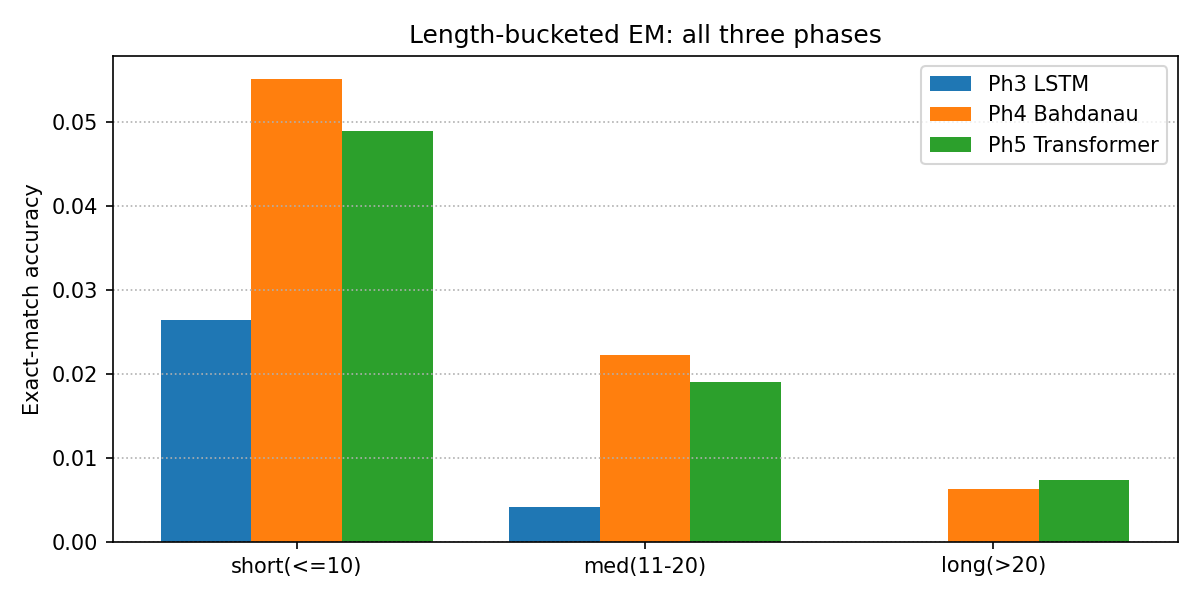
\includegraphics[width=0.72\textwidth]{../evaluation/phase5_transformer/three_way_compare.png}
\caption{Length-bucketed exact match for all three correction models. The
bottleneck LSTM (blue) drops to near zero on medium/long sentences; the
Transformer (green) overtakes Bahdanau (orange) on the long bucket.}
\label{fig:lenbucket}
\end{figure}

\subsection{Attention visualisations}
The attention weights are directly interpretable. Figure~\ref{fig:attn} shows
three views for the same test sentence (\emph{``Why new record is taking so
long.''}): the Bahdanau decoder alignment, the Transformer's encoder
self-attention, and the Transformer's decoder cross-attention. Bright cells mark
which source tokens are focused on while producing each output token.

The Bahdanau and Transformer cross-attention maps (a, c) are the most directly
comparable --- both align decoder output positions to source positions. Both are
diagonal-dominant, confirming a sensible, mostly monotonic source-to-target
alignment, with off-diagonal mass exactly where a word is inserted: in panel (c)
the inserted article \texttt{\_the} draws attention onto the neighbouring
\texttt{\_new}/\texttt{\_record} tokens. The encoder self-attention (b) instead
shows tokens attending \emph{within} the source to build context. The key
qualitative point: the LSTM with attention and the Transformer learn
\emph{visually similar alignments} --- a first hint at why their scores are so
close (Section~\ref{sec:close}).

\begin{figure}[h]
\centering
\begin{subfigure}{0.32\textwidth}
  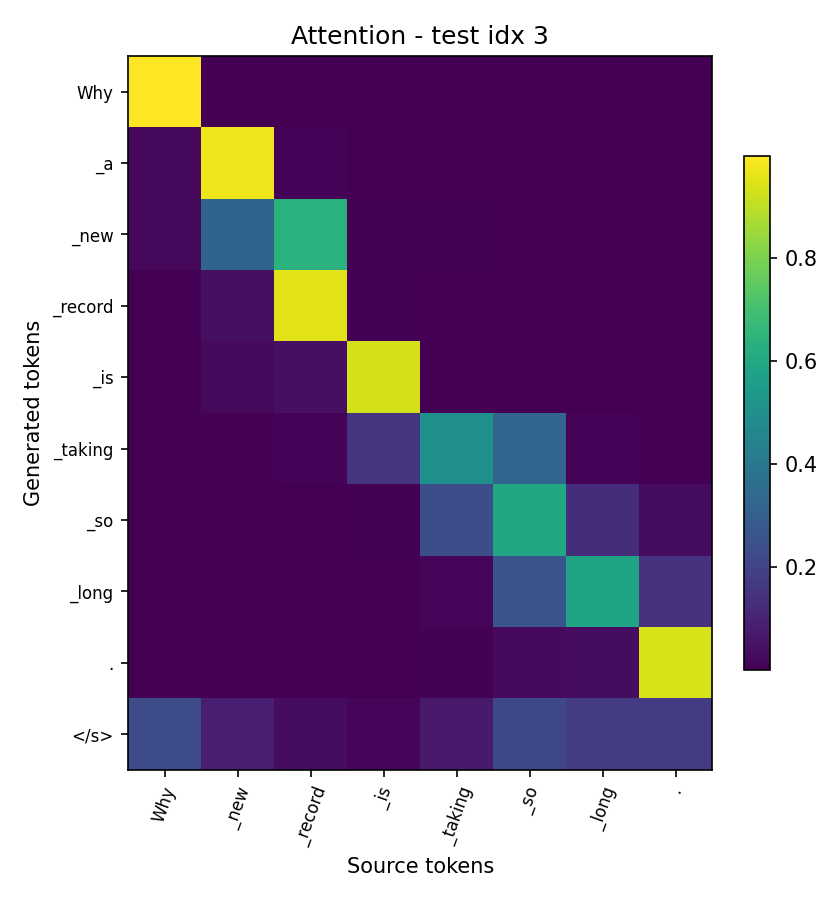
\includegraphics[width=\textwidth]{figures/attn_3.png}
  \caption{Bahdanau decoder alignment.}
\end{subfigure}\hfill
\begin{subfigure}{0.32\textwidth}
  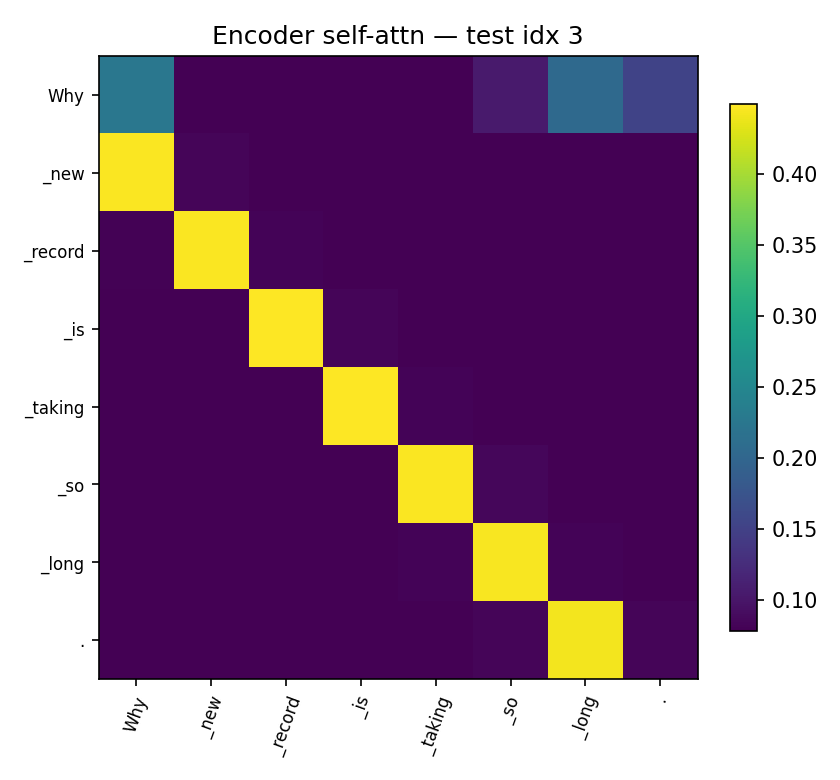
\includegraphics[width=\textwidth]{../evaluation/phase5_transformer/enc_self_attn_3.png}
  \caption{Transformer encoder self-attention.}
\end{subfigure}\hfill
\begin{subfigure}{0.32\textwidth}
  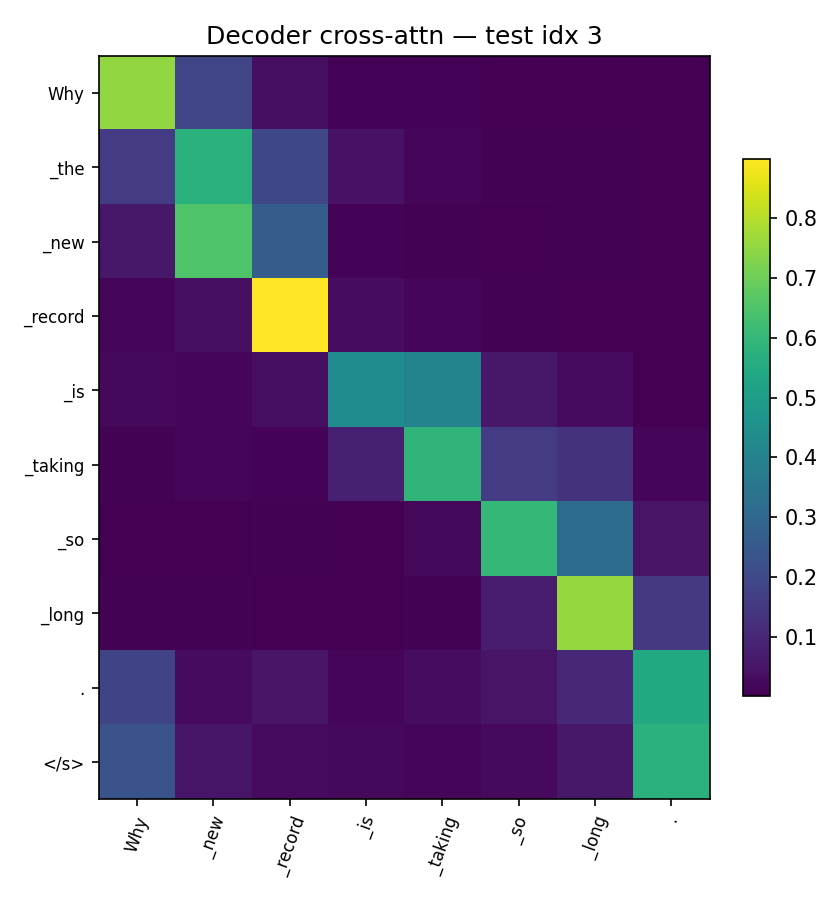
\includegraphics[width=\textwidth]{../evaluation/phase5_transformer/dec_cross_attn_3.png}
  \caption{Transformer decoder cross-attention.}
\end{subfigure}
\caption{Attention is interpretable: each cell shows how much one token attends
to another. (a) and (c) are the analogous source-to-output alignments of the
two attention models.}
\label{fig:attn}
\end{figure}

% ------------------------------------------------------------------
\subsection{Worked examples: the three correctors side by side}
Aggregate scores hide \emph{how} the models behave. Below are two test
sentences with the source, the reference, and each model's greedy prediction.

\paragraph{Example A --- a short sentence (test index 3).}
\begin{lstlisting}
SRC : Why new record is taking so long.
REF : Why the new record is taking so long.   (insert the article "the")
P3  : Why new record is taking so long.        LSTM       - no edit (copies source)
P4  : Why a new record is taking so long.      Bahdanau   - inserts an article ("a")
P5  : Why new record is taking so long?        Transformer- changes "." to "?"
\end{lstlisting}
The LSTM makes \emph{no} correction at all. Bahdanau correctly identifies that
an article is missing and inserts one --- it picks \texttt{a} where the
reference wants \texttt{the}, so it still scores EM\,=\,0, but the \emph{type}
of edit is right. The Transformer makes a different, defensible edit
(declarative $\rightarrow$ question mark). All three miss the exact reference,
yet only the two attention models attempt a real correction.

\paragraph{Example B --- a long, noisy sentence (test index 102).}
\begin{lstlisting}
SRC : ... you will need to come to bp.co.uk/driveindineout and got your meal
      code for PizzaExpress full T&C is here.
REF : ... you will need to visit bp.co.uk/driveindineout and get your meal
      code for PizzaExpress. Full T&Cs are here ...
P3  : ... you need to be cpue to buy and/indukine stead. However, if your
      meal made for Pax code ...               <- hallucinated nonsense
P4  : ... come to bp.co.uk/driveindoutout and got your meal code ...
                                                <- copies, corrupts the URL
P5  : ... come to bp.co.uk/driveindineout and get your meal code ...
                                                <- copies, fixes "got" -> "get"
\end{lstlisting}
On a long sentence the bottleneck LSTM loses the thread entirely and
hallucinates. Both attention models instead play it safe and largely copy the
source --- but the Transformer lands the one genuine grammatical fix
(\texttt{got}$\rightarrow$\texttt{get}) while Bahdanau introduces a spurious
change to the URL. This is the \emph{typical} P4-vs-P5 difference: small, a
token or two, not dramatic.

% ------------------------------------------------------------------
\subsection{Why the attention LSTM and the Transformer are so close}
\label{sec:close}
The headline test GLEU is effectively tied (0.618 for both beam-4 results), and
the worked examples above show why the gap is small. There are four reasons:

\begin{enumerate}[noitemsep]
  \item \textbf{The decisive feature is shared.} The project's largest jump
        (+0.386 GLEU) came from giving the decoder \emph{full access to the
        source} via attention. \emph{Both} Model 3 and Model 4 already have
        this. The remaining LSTM-vs-self-attention difference is a
        second-order effect on top of the same key idea.
  \item \textbf{Both hit the data ceiling, not their capacity ceiling.} Trained
        on the same one-million-pair budget, the same noisy C4\_200M
        references, and the same tokenizer, both models converge to the
        corpus's effective GLEU ceiling ($\approx$0.62). The binding
        constraint is reference quality (Section~\ref{sec:challenge}), not
        architecture --- a constraint a bigger or different model cannot lift.
  \item \textbf{C4\_200M sentences are mostly short.} The Transformer's
        signature advantage --- an $O(1)$ path between any two tokens --- only
        pays off when dependencies are long. Most web sentences here are short
        enough that the LSTM's sequential path is not a real handicap.
        Figure~\ref{fig:lenbucket} confirms this: the two models only diverge
        in the \emph{long} bucket, where the Transformer wins.
  \item \textbf{The worked examples agree.} On hard inputs both models fall
        back to conservative copying; their outputs differ by only one or two
        tokens.
\end{enumerate}

So the Transformer does not \emph{out-score} the attention LSTM here --- it
\emph{matches} it. Its real victory is efficiency: the same quality with
\textbf{8.05\,M parameters instead of 29.06\,M} ($3.6\times$ fewer) and far
faster, fully parallel training. That efficiency is what would let it pull
ahead given more data, more epochs, or a cleaner corpus --- none of which this
project's fixed budget and noisy references provide.

% =====================================================================
\section{Grammar-Rule-Based Analysis of Outputs}
% =====================================================================
Beyond aggregate scores, we inspected the predictions rule by rule. Each test
row is a triple \texttt{(source, hypothesis, reference)}. We grouped corrections
into standard GEC error categories and summarise the qualitative findings below.

\paragraph{Subject--verb agreement.}
Handled well by both attention models.
\begin{lstlisting}
SRC: What are this job about?
HYP: What is this job about?     (Transformer - correct)
\end{lstlisting}
The model attends from the verb back to the subject and fixes \texttt{are}
$\rightarrow$ \texttt{is}. The bottleneck LSTM frequently misses agreement once
the subject is far from the verb.

\paragraph{Articles and determiners.}
Insertion of missing articles is among the most common successful edits:
\begin{lstlisting}
SRC: Why new record is taking so long.
REF: Why the new record is taking so long.
\end{lstlisting}
The Transformer reliably inserts \texttt{the/a}; it occasionally over-corrects
by adding an article where the reference has none.

\paragraph{Verb tense and inflection.}
Tense fixes (\texttt{go}$\rightarrow$\texttt{went}) and gerund/participle
inflection (\texttt{learning}$\rightarrow$\texttt{learned}) succeed when a tense
cue (e.g.\ \texttt{yesterday}) is present in the sentence; self-attention links
the verb to that cue directly.

\paragraph{Punctuation and spacing.}
Sentence-final punctuation and missing spaces are corrected often:
\begin{lstlisting}
SRC: 25% off Generation Brands Lighting and-Home Decor.
REF: 25% off Generation Brands Lighting and Home Decor.
\end{lstlisting}

\paragraph{Spelling / rare words.}
Mixed. Because rare words are split into BPE subwords, the models can repair
some misspellings but also \emph{hallucinate} on very rare tokens --- the
LSTM+Bahdanau output for one medical sentence produced the non-word
``Arasemiaia'' where the reference had ``thalassemia''.

\paragraph{Failure mode --- conservative copying.}
The most frequent error is \emph{under-correction}: the model copies the source
unchanged when the required edit is non-local or semantic. This is rational
under cross-entropy --- copying is the safe, high-probability action --- but it
caps recall.

\paragraph{Summary.} Local, syntactic rules (agreement, articles, tense,
punctuation) are learned well by the attention models. Long-range, semantic, or
lexical-choice edits remain hard, and the models prefer to copy rather than risk
a wrong correction.

% =====================================================================
\section{The ``Final Challenge'' and Dataset Quality}
\label{sec:challenge}
% =====================================================================
The Final Challenge asks why \emph{every} model --- including the strongest
Transformer --- scores only $\sim$2\,\% exact match, and whether this reflects
the models or the data. Direct inspection of \texttt{(source, hypothesis,
reference)} triples gives a clear answer: the ceiling is set by
\textbf{reference quality}, not model capacity.

\paragraph{1. References are paraphrases, not minimal corrections.}
\begin{lstlisting}
SRC: ... investors have informed that the Internet startups that they fund
     can't afford a "commercially reasonable" price for bandwidth!
REF: ... investors suggest that the Internet start-ups they fund
     can't afford a "commercially reasonable" price for bandwidth!
\end{lstlisting}
\texttt{informed}$\rightarrow$\texttt{suggest} and \texttt{startups}$\rightarrow$
\texttt{start-ups} are stylistic rewrites, not grammatical errors. A model that
correctly fixes only the grammar can \emph{never} match this reference, so EM is
artificially near zero.

\paragraph{2. Some references contain errors themselves.}
The C4\_200M corruption pipeline is automatic and noisy. Observed targets
include non-words:
\begin{lstlisting}
SRC: ... no sleep = no brain workout.
REF: ... no sleep = no brain worky.        <-- "worky" is not a word
\end{lstlisting}
Here the ``clean'' reference is itself broken. Training on such pairs teaches
the model nothing useful and penalises a correct output.

\paragraph{3. Multiple valid corrections exist.}
A single ungrammatical sentence usually has several acceptable corrections.
EM credits exactly one. This is a known weakness of EM for GEC and the reason
GLEU and $F_{0.5}$ --- which reward n-gram overlap rather than exact identity ---
are the meaningful metrics here.

\paragraph{Implications.}
\begin{itemize}[noitemsep]
  \item Exact match should be reported but not optimised; GLEU/$F_{0.5}$ are the
        trustworthy signals.
  \item The synthetic corruption used in C4\_200M does not always preserve
        meaning, so the corpus mixes genuine GEC pairs with paraphrase and
        noise pairs.
  \item A realistic upper bound for EM on this corpus is far below 100\,\%; the
        observed 2--3\,\% is consistent with models that correct grammar
        correctly but cannot reproduce arbitrary paraphrases.
  \item Cleaner data (human-verified references, or filtering pairs whose edit
        distance is implausibly large) would likely improve every metric more
        than additional model capacity would.
\end{itemize}

% =====================================================================
\section{Conclusion}
% =====================================================================
We built and compared four models for Grammatical Error Correction on a
one-million-pair subset of C4\_200M under a shared tokenizer and data budget.

\begin{itemize}[noitemsep]
  \item The \textbf{Bag-of-Words} baseline detects grammaticality at only
        $\sim$62\,\% accuracy and cannot correct text --- establishing the lower
        bound.
  \item The \textbf{LSTM encoder--decoder} corrects sentences but is limited by
        the fixed-size bottleneck (GLEU 0.213 greedy).
  \item \textbf{Bahdanau attention} is the single most important improvement,
        raising greedy GLEU to 0.599 by letting the decoder re-query the full
        source.
  \item The \textbf{Transformer} matches the attention LSTM on the test set
        (GLEU $\approx$0.618), achieves the best validation GLEU (0.613), and
        does so with $3.6\times$ fewer parameters and far faster training.
\end{itemize}

The grammar-rule analysis shows the models reliably learn local syntactic rules
(agreement, articles, tense, punctuation) but under-correct long-range and
lexical edits. The Final Challenge discussion shows the binding constraint is
\textbf{dataset quality}: C4\_200M references are frequently paraphrases or
contain noise, which caps exact match near 2\,\% regardless of architecture.

\paragraph{Future work.} Filtering noisy pairs by edit distance, training for
more epochs, increasing Transformer depth toward the 6-layer original, adding a
KV-cache for faster beam search, and evaluating on a human-curated GEC test set
(e.g.\ CoNLL-2014 or BEA-2019) would all sharpen the picture beyond what the
synthetic corpus allows.

% =====================================================================
\section*{References}
% =====================================================================
\begin{enumerate}[noitemsep,leftmargin=2em]
  \item Sutskever, Vinyals, Le. \emph{Sequence to Sequence Learning with Neural
        Networks}. NeurIPS 2014.
  \item Bahdanau, Cho, Bengio. \emph{Neural Machine Translation by Jointly
        Learning to Align and Translate}. ICLR 2015.
  \item Hochreiter, Schmidhuber. \emph{Long Short-Term Memory}. Neural
        Computation 1997.
  \item Vaswani et al. \emph{Attention Is All You Need}. NeurIPS 2017.
  \item Napoles et al. \emph{Ground Truth for Grammatical Error Correction
        Metrics (GLEU)}. ACL 2015.
  \item Stahlberg, Kumar. \emph{Synthetic Data Generation for Grammatical Error
        Correction with Tagged Corruption Models (C4\_200M)}. BEA 2021.
\end{enumerate}

\end{document}
